\section{Addierer (Konstante)}
\label{sec:knf:konstadd}

Für die Addition der Rundenkonstanten wird eine Addition konstruiert, die Literale für die Konstanten vermeidet.
Da die Konstanten bekannt sind, können der Halbaddierer, der Volladdierer und der Mod-2 Addierer entsprechend reduziert werden.
Abbildung \ref{fig:adder_reduced} zeigt die reduzierten Varianten. In der ersten Zeile der Tabelle sind die Varianten dargestellt,
die genutzt werden, falls das eigehende Bit (b) der Konstante den Wert $0$ hat. Entsprechend sind in der zweiten Zeile die Varianten für ein
Bit (b) mit dem Wert $1$ dargestellt.
\begin{figure}[!h]
  \centering
  \begin{tabular}{r|c|c|c}
    \hiderowcolors
    b & Halbaddierer                                 & Volladdierer                                 & Mod-2 Addierer\\
    \hline
    0 & \begin{minipage}{0.29\textwidth}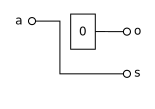
\includegraphics[scale=1]{images/halfadder0}\end{minipage} & \begin{minipage}{0.29\textwidth}\includegraphics[scale=1]{images/fulladder0}\end{minipage} & \begin{minipage}{0.29\textwidth}\includegraphics[scale=1]{images/lastadder0}\end{minipage}\\
    \hline
    1 & \begin{minipage}{0.29\textwidth}\includegraphics[scale=1]{images/halfadder1}\end{minipage} & \begin{minipage}{0.29\textwidth}\includegraphics[scale=1]{images/fulladder1}\end{minipage} & \begin{minipage}{0.29\textwidth}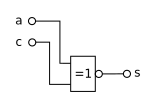
\includegraphics[scale=1]{images/lastadder1}\end{minipage}\\
    \showrowcolors
  \end{tabular}
  \caption[Reduziert Addierer]{Reduzierte Addierer\protect\footnotemark}
  \label{fig:adder_reduced}
\end{figure}
\footnotetext{Jeweils auf Basis von MovGP0, CC BY-SA 2.0 de, \url{https://commons.wikimedia.org/w/index.php?curid=22912775}}

Ein Halbaddierer der zwei Bits addiert und dem Eingang (b) den Wert $0$ erhält, gibt den Wert des Eingangs (a) direkt an die Summe (s) weiter.
Der Übertrag (o) kann dabei niemals $1$ werden. Hat der Eingang (b) den Wert $1$, liegt immer genau dann ein Übertrag (o) vor, wenn am Eingang (a)
der Wert $1$ anliegt. Die Summe (s) hat jedoch nur den Wert $1$, falls der Wert $0$ am Eingang (a) anliegt. Der Eingang (a) muss invertiert werden.

Der Volladdierer addiert drei Bits. Liegt dabei an einem beliebigen Eingang ein Bit mit dem Wert $0$ an, brauchen nur noch zwei Bits addiert werden.
Der Volladdierer kann auf einen Halbaddierer reduziert werden. Liegt am Eingang (b) der Wert $1$ an, ist für einen Übertrag nur noch Vorraussetzung,
das Eingang (a) oder Übertrag (c) den Wert $1$ haben. Für die Summe (s) liegt durch den Eingang (b) schon ein $1$-Bit vor. Die Summe (s) ist nur dann
$1$, wenn der Eingang(a) und der Übertrag (c) gleich sind, was sich durch den inversen XOR-Operator beschreiben lässt.

Die Mod-2 Addierer werden, wie schon in Abschnitt \ref{sec:grundlagen_add} durchgeführt, aus den Volladdierern erzeugt, indem die für den Übertrag
notwendigen Operatoren entfernt werden.

Nach der Erstellung der reduzierten Addierer, werden die konjunktiven Normalformen erstellt. Wie auch im vorhergehenden Abschnitt werden zwei mögliche
Lösungen generiert, um eine optimale Lösung sowohl mit, als auch ohne XOR-Unterstützung bereit zu stellen. eqntott und Espresso werden dabei nicht mit
einbezogen, da alle Ausgänge direkt durch jeweils ein Gatter aus den Eingängen berechnet werden. \TODO{überarbeiten - stimmt nicht}

\TODO{erledigen}

\begin{figure}[!h]
  \centering
  \begin{minipage}[c]{0.3cm}
    ~
  \end{minipage}
  \begin{minipage}[c]{7.1cm}
    ~~~~~~~~~~~~~~~~~~~~~~~~~~~~~~~~b = $0$
  \end{minipage}
  \begin{minipage}[c]{7cm}
    ~~~~~~~~~~~~~~~~~~~~~~~~~~~~~~~~b = $1$
  \end{minipage}
  \begin{minipage}[l]{0.4cm}
    ~
  \end{minipage}
  \begin{minipage}[l]{3.5cm}
    \underline{Ohne XOR}\\
    ~\\
    \underline{Übertrag - $0$}\\
    $ (\overline{o}) ~ \wedge $\\
    ~\\
    \underline{Summe - EQ}\\
    $ (\overline{s} \vee  a) ~ \wedge $\\
    $ (s \vee \overline{a}) $
  \end{minipage}
  \begin{minipage}[l]{3.5cm}
    \underline{Mit XOR}\\
    ~\\
    \underline{Übertrag - $0$}\\
    $ (\overline{o}) ~ \wedge $\\
    ~\\
    \underline{Summe - EQ}\\
    $ (\overline{s} \veebar a) $\\
    ~
  \end{minipage}
  \begin{minipage}[l]{3.5cm}
    \underline{Ohne XOR}\\
    ~\\
    \underline{Übertrag - EQ}\\
    $ (\overline{o} \vee  a) ~ \wedge $\\
    $ (o \vee \overline{a}) ~ \wedge $\\
    \underline{Summe - NOT}\\
    $ (s \vee  a) ~ \wedge $\\
    $ (\overline{s} \vee \overline{a}) $
  \end{minipage}
  \begin{minipage}[l]{3.5cm}
    \underline{Mit XOR}\\
    ~\\
    \underline{Übertrag - EQ}\\
    $ (\overline{o} \veebar a) ~ \wedge $\\
    ~\\
    \underline{Summe - NOT}\\
    $ (s \veebar a) $\\
    ~
  \end{minipage}
  \caption{Reduzierter Halbaddierer - Konjuktive Normalform}
  \label{fig:red_halfadder_cnf}
\end{figure}

\begin{figure}[!h]
  \centering
  \begin{minipage}[c]{0.3cm}
    ~
  \end{minipage}
  \begin{minipage}[c]{7.1cm}
    ~~~~~~~~~~~~~~~~~~~~~~~~~~~~~~~~b = $0$
  \end{minipage}
  \begin{minipage}[c]{7cm}
    ~~~~~~~~~~~~~~~~~~~~~~~~~~~~~~~~b = $1$
  \end{minipage}
  \begin{minipage}[l]{0.4cm}
    ~
  \end{minipage}
  \begin{minipage}[l]{3.5cm}
    \underline{Ohne XOR}\\
    ~\\
    $ (\overline{s} \vee a \vee c) ~ \wedge $\\
    $ (\overline{o} \vee \overline{s}) ~ \wedge $\\
    $ (\overline{o} \vee c) ~ \wedge $\\
    $ (o \vee \overline{a} \vee \overline{c}) ~ \wedge $\\
    $ (s \vee a \vee \overline{c}) ~ \wedge $\\
    $ (s \vee \overline{a} \vee c) $
  \end{minipage}
  \begin{minipage}[l]{3.5cm}
    \underline{Mit XOR}\\
    ~\\
    \underline{Übertrag - AND}\\
    $ (\overline{o} \vee a) ~ \wedge $\\
    $ (\overline{o} \vee c) ~ \wedge $\\
    $ (o \vee \overline{a} \vee \overline{c}) ~ \wedge $\\
    \underline{Summe - XOR}\\
    $ (\overline{s} \veebar a \veebar c) $
  \end{minipage}
  \begin{minipage}[l]{3.5cm}
    \underline{Ohne XOR}\\
    ~\\
    Err\\
    ~\\
    ~\\
    ~\\
    ~\\
    ~
  \end{minipage}
  \begin{minipage}[l]{3.5cm}
    \underline{Mit XOR}\\
    ~\\
    \underline{Übertrag - OR}\\
    $ (o \vee \overline{a}) ~ \wedge $\\
    $ (o \vee \overline{c}) ~ \wedge $\\
    $ (\overline{o} \vee a \vee c) ~ \wedge $\\
    \underline{Summe - XNOR}\\
    $ (s \veebar a \veebar c) $
  \end{minipage}
  \caption{Reduzierter Volladdierer - Konjuktive Normalform}
  \label{fig:red_fulladder_cnf}
\end{figure}

\begin{figure}[!h]
  \centering
  \begin{minipage}[c]{0.3cm}
    ~
  \end{minipage}
  \begin{minipage}[c]{7.1cm}
    ~~~~~~~~~~~~~~~~~~~~~~~~~~~~~~~~b = $0$
  \end{minipage}
  \begin{minipage}[c]{7cm}
    ~~~~~~~~~~~~~~~~~~~~~~~~~~~~~~~~b = $1$
  \end{minipage}
  \begin{minipage}[l]{0.4cm}
    ~
  \end{minipage}
  \begin{minipage}[l]{3.5cm}
    \underline{Ohne XOR}\\
    ~\\
    \underline{Summe - XOR}\\
    $ (\overline{s} \vee \overline{a} \vee \overline{c}) ~ \wedge $\\
    $ (s \vee a \vee \overline{c}) ~ \wedge $\\
    $ (s \vee \overline{a} \vee c) ~ \wedge $\\
    $ (\overline{s} \vee a \vee c) $
  \end{minipage}
  \begin{minipage}[l]{3.5cm}
    \underline{Mit XOR}\\
    ~\\
    \underline{Summe - XOR}\\
    $ (\overline{s} \veebar a \veebar c) $\\
    ~\\
    ~\\
    ~
  \end{minipage}
  \begin{minipage}[l]{3.5cm}
    \underline{Ohne XOR}\\
    ~\\
    \underline{Summe - XNOR}\\
    $ (s \vee \overline{a} \vee \overline{c}) ~ \wedge $\\
    $ (\overline{s} \vee a \vee \overline{c}) ~ \wedge $\\
    $ (\overline{s} \vee \overline{a} \vee c) ~ \wedge $\\
    $ (s \vee a \vee c) $
  \end{minipage}
  \begin{minipage}[l]{3.5cm}
    \underline{Mit XOR}\\
    ~\\
    \underline{Summe - XNOR}\\
    $ (s \veebar a \veebar c) $\\
    ~\\
    ~\\
    ~
  \end{minipage}
  \caption{Reduzierter Mod-2 Addierer - Konjuktive Normalform}
  \label{fig:red_lastadder_cnf}
\end{figure}

\TODO{erledigen}